\documentclass[../poliXuniversity_hospital_(USP)_report.tex]{subfiles}

\begin{document}
\chapter{Arquitetura do Projeto}

Tanto a Hema Bot, quanto o Golgi Bot e Ciclo Êrgometro seguem a mesma estrutura, que é composta por três núcleos. O Eletrônico, Mecânico e Computacional, cada um responsável pelo desenvolvimento de cada subsistema dos equipamentos e pela integração entre hardware e software de maneira funcional.

\subsection{Sistema Mecânico}

É responsável por realizar toda concepção da estrutura e mecanismos através da modelagem 3D, manufatura de peças, prototipação e manutenção dos projetos. A equipe utiliza e domina softwares CAD de simulação para concepção "virtual", ferramentas como furadeiras, impressoras 3D, esmelhiradeira e entre outras para a manufatura mecânica e também realiza a avaliação e contratação de serviços de usinagem e soldagem. Todas tarefas de prototipagem são realizadas presencialmente no laboratório da ZIMA pelos seus integrantes.

\subsection{Sistema Eletrônico}

Destinado a concepção dos módulos embarcados, fornecimento de energia, sensoriamento e sistema de tração e para isso utiliza Softwares como Altium Designer e NSIM. Além disso é realizado a soldagem das placas de circuito impresso, cabeamento, manutenção eletrônica e compra e contratação de serviços/equipamentos eletrônicos.

\subsection{Sistema Computacional}

Encarregado desenvolver, simular e validar todo software usado nos microcontroladores ou computadores embarcados. Para isso, o dominio de ferramentas de versionamento como Git\cite{git21} e GitHub\cite{github21} são amplamente utilizados pela equiepebem como as linguagens \cite{c++21}, \cite{python21} e frameWorks de simulação como ROS \cite{ROS21}, Rviz\cite{rviz21} e Gazebo\cite{gazebo21}. Além de embarcados e simulações, sistemas de interação com usuario também são feitos pela computação. Mais recentemente, a equipe adicionou a área de Desenvolvimento Web e Mobile, responsável pela criação e manutenção do site da zimausp.org e do aplicatovo do Hema Bot.

\begin{figure}[h]
\centering
    \begin{minipage}{0.5\textwidth}
        \centering
        \caption{Fusion 360}
        \centering % para centralizarmos a figura
        
\includegraphics[width=7cm]{images/logo_fusion.png}
        \caption*{Fonte: Autodesk}
        \label{figura: Fusion 360}
        
    \end{minipage}\hfill
    \begin{minipage}{0.5\textwidth}
    
        \centering
        \caption{Altium Designer}
        \centering % para centralizarmos a figura
        
\includegraphics[width=5cm]{images/logo_altium.png}
        \caption*{Fonte: Altium}
        \label{figura:Altium Designer}
        
    \end{minipage}\hfill
\end{figure}

\begin{figure}[h]
\centering
    \begin{minipage}{0.5\textwidth}
        \centering
        \caption{Gazebo}
        \centering % para centralizarmos a figura
        
\includegraphics[width=3cm]{images/gazebo.png}
        \caption*{Fonte: Gazebo}
        \label{figura: Gazebo}
        
    \end{minipage}\hfill
    \begin{minipage}{0.5\textwidth}
    
        \centering
        \caption{Robot Operating system (ROS)}
        \centering % para centralizarmos a figura
        
\includegraphics[width=5cm]{images/logo_ros.png}
        \caption*{Fonte: Ros}
        \label{figura:Altium Designer}
        
    \end{minipage}\hfill
\end{figure}

\begin{figure}[h]
\centering
    \begin{minipage}{0.5\textwidth}
        \centering
        \caption{Github}
        \centering % para centralizarmos a figura
        
\includegraphics[width=4cm]{images/logo_git.png}
        \caption*{Fonte: Github}
        \label{figura: Github}
        
    \end{minipage}\hfill
    \begin{minipage}{0.5\textwidth}
    
        \centering
        \caption{Rviz}
        \centering % para centralizarmos a figura
        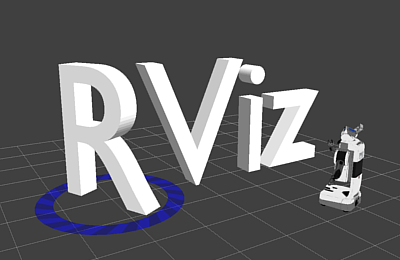
\includegraphics[width=5cm]{images/logo_rviz.png}
        \caption*{Fonte: github}
        \label{figura:Rviz}
        
    \end{minipage}\hfill
\end{figure}

\end{document}